\appendix

\chapter{Appendix A - Grafici FEMNIST}
Quella che segue è una lista dei grafici di tutti gli esperimenti
che sono stati svolti sul dataset FEMNIST con ottimizzazione SGD.
La colonna di sinistra 
riporta i risultati ottenuti con il metodo \texttt{share-disjoint}, 
quella di destra \texttt{unify}.
\begin{figure}[htbp]  % h: here, t: top, b: bottom, p: page
    \centering
    \begin{subfigure}[b]{0.47\textwidth}
        \centering
        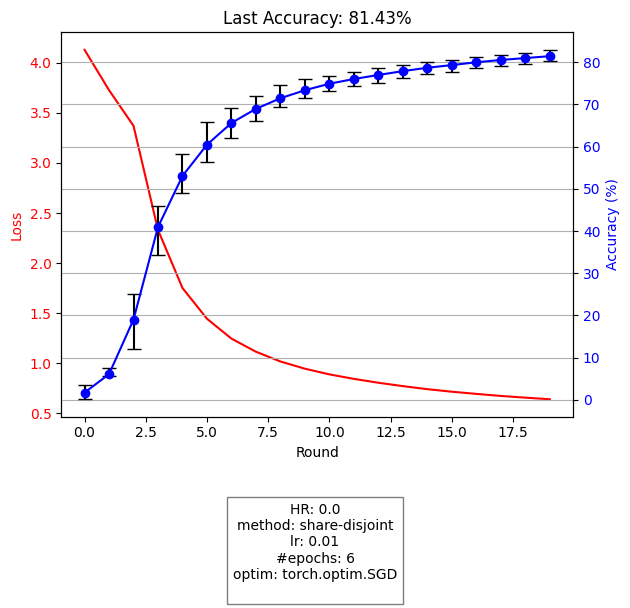
\includegraphics[width=\textwidth]{../plots/femnist-horizontal/sgd/results-h0_0-hm_share-disjoint-lr0_01-e6-torch_optim_SGD.png}
    \end{subfigure}
    \hfill
    \begin{subfigure}[b]{0.47\textwidth}
        \centering
        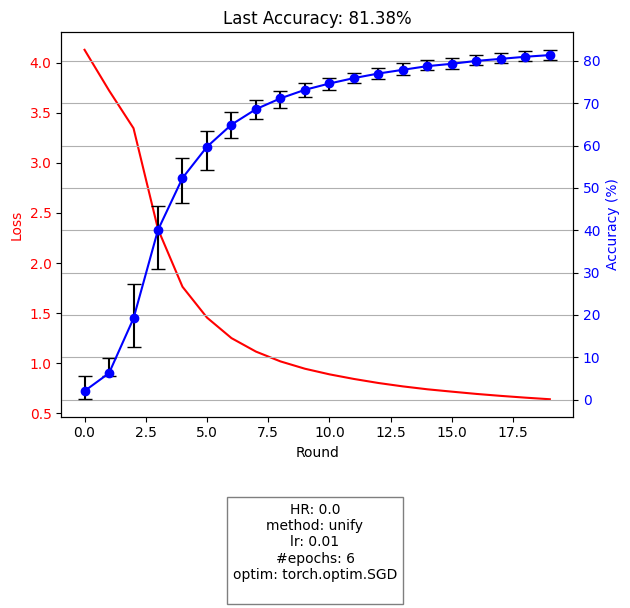
\includegraphics[width=\textwidth]{../plots/femnist-horizontal/sgd/results-h0_0-hm_unify-lr0_01-e6-torch_optim_SGD.png}
    \end{subfigure}
\end{figure}
\begin{figure}[htbp]  % h: here, t: top, b: bottom, p: page
    \centering
    \begin{subfigure}[b]{0.47\textwidth}
        \centering
        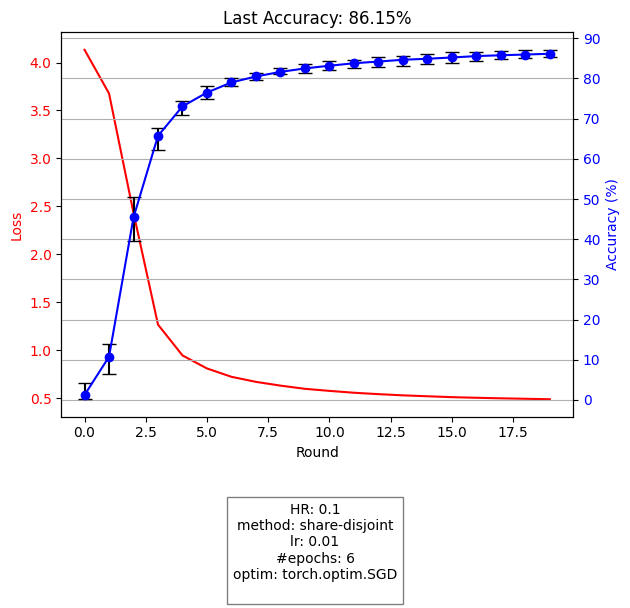
\includegraphics[width=\textwidth]{../plots/femnist-horizontal/sgd/results-h0_1-hm_share-disjoint-lr0_01-e6-torch_optim_SGD.png}
    \end{subfigure}
    \hfill
    \begin{subfigure}[b]{0.47\textwidth}
        \centering
        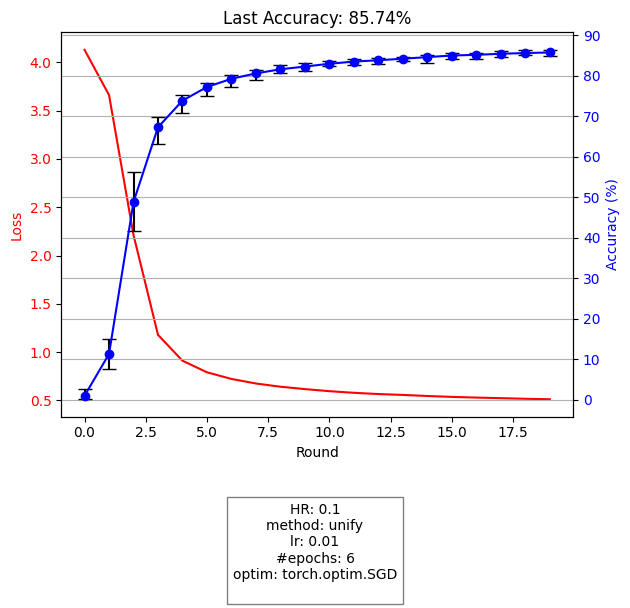
\includegraphics[width=\textwidth]{../plots/femnist-horizontal/sgd/results-h0_1-hm_unify-lr0_01-e6-torch_optim_SGD.png}
    \end{subfigure}
\end{figure}
\begin{figure}[htbp]  % h: here, t: top, b: bottom, p: page
    \centering
    \begin{subfigure}[b]{0.47\textwidth}
        \centering
        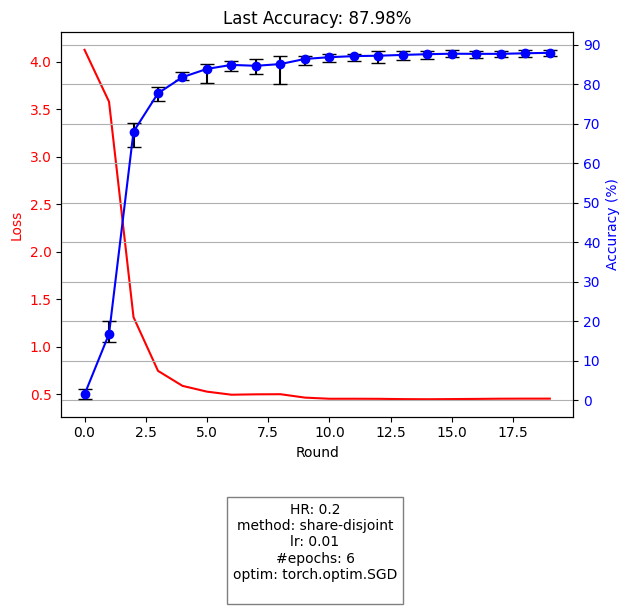
\includegraphics[width=\textwidth]{../plots/femnist-horizontal/sgd/results-h0_2-hm_share-disjoint-lr0_01-e6-torch_optim_SGD.png}
    \end{subfigure}
    \hfill
    \begin{subfigure}[b]{0.47\textwidth}
        \centering
        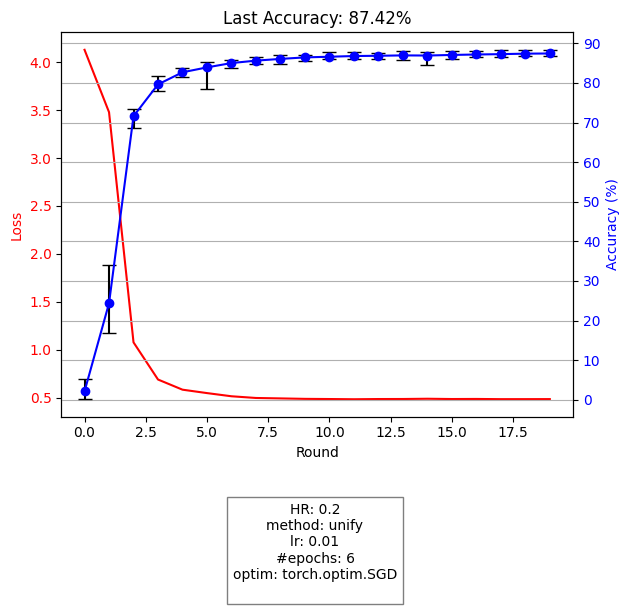
\includegraphics[width=\textwidth]{../plots/femnist-horizontal/sgd/results-h0_2-hm_unify-lr0_01-e6-torch_optim_SGD.png}
    \end{subfigure}
\end{figure}
\begin{figure}[htbp]  % h: here, t: top, b: bottom, p: page
    \centering
    \begin{subfigure}[b]{0.47\textwidth}
        \centering
        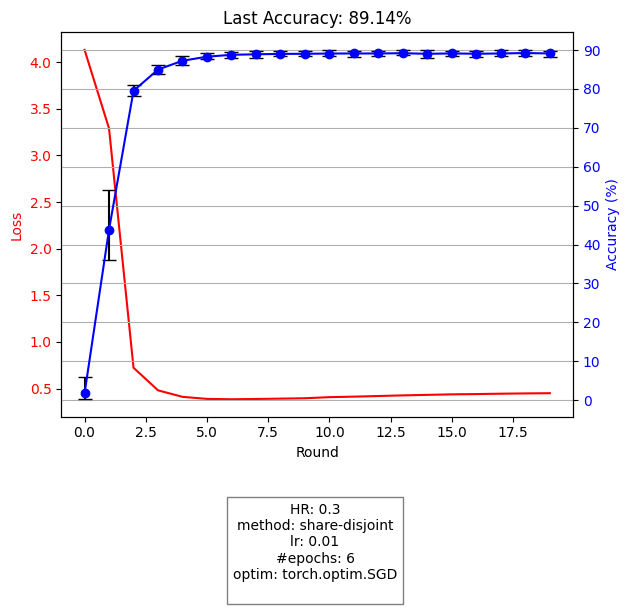
\includegraphics[width=\textwidth]{../plots/femnist-horizontal/sgd/results-h0_3-hm_share-disjoint-lr0_01-e6-torch_optim_SGD.png}
    \end{subfigure}
    \hfill
    \begin{subfigure}[b]{0.47\textwidth}
        \centering
        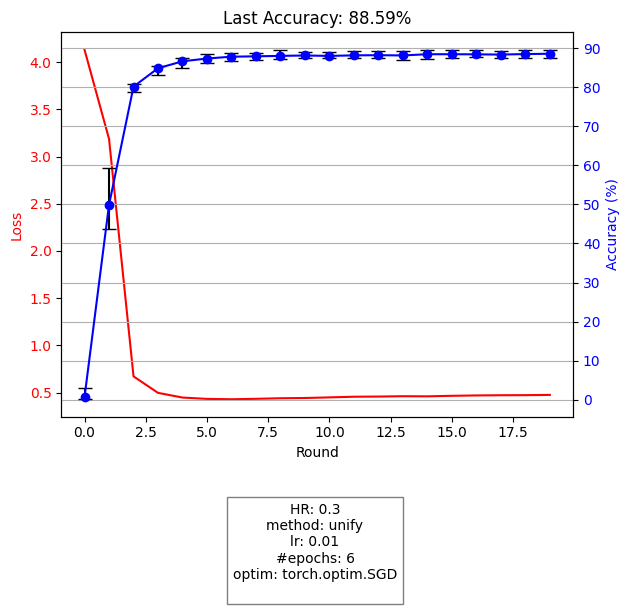
\includegraphics[width=\textwidth]{../plots/femnist-horizontal/sgd/results-h0_3-hm_unify-lr0_01-e6-torch_optim_SGD.png}
    \end{subfigure}
\end{figure}
\begin{figure}[htbp]  % h: here, t: top, b: bottom, p: page
    \centering
    \begin{subfigure}[b]{0.47\textwidth}
        \centering
        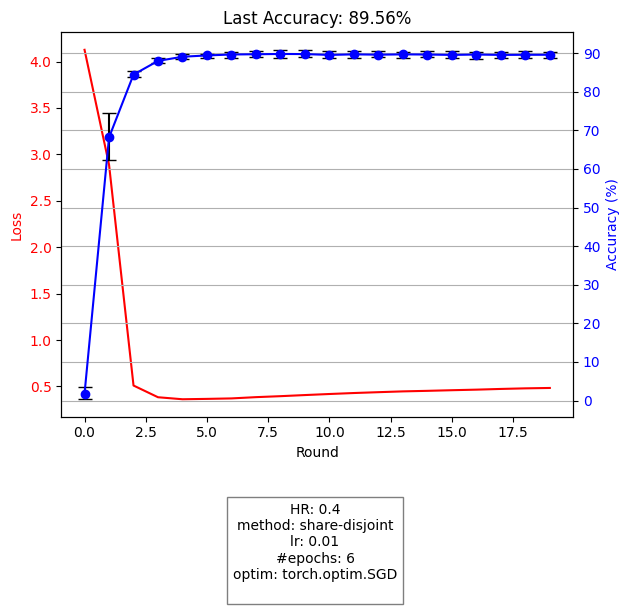
\includegraphics[width=\textwidth]{../plots/femnist-horizontal/sgd/results-h0_4-hm_share-disjoint-lr0_01-e6-torch_optim_SGD.png}
    \end{subfigure}
    \hfill
    \begin{subfigure}[b]{0.47\textwidth}
        \centering
        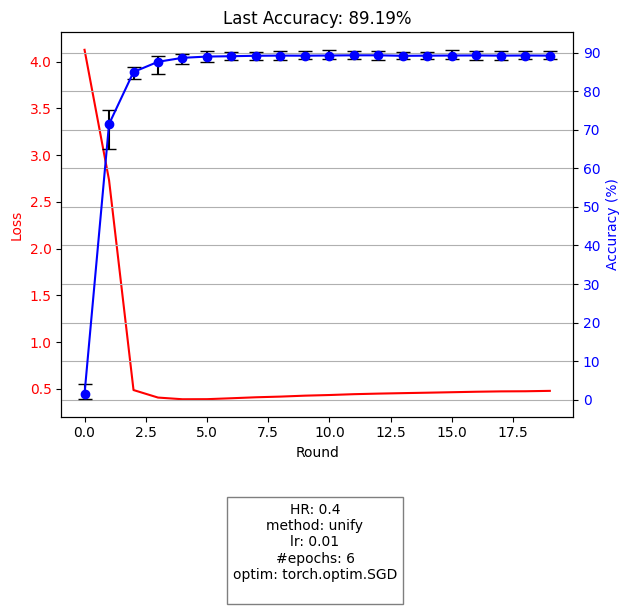
\includegraphics[width=\textwidth]{../plots/femnist-horizontal/sgd/results-h0_4-hm_unify-lr0_01-e6-torch_optim_SGD.png}
    \end{subfigure}
\end{figure}
\begin{figure}[htbp]  % h: here, t: top, b: bottom, p: page
    \centering
    \begin{subfigure}[b]{0.47\textwidth}
        \centering
        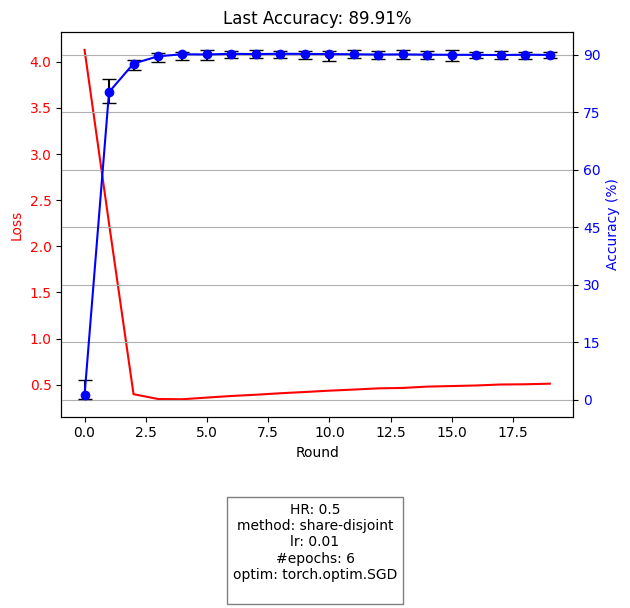
\includegraphics[width=\textwidth]{../plots/femnist-horizontal/sgd/results-h0_5-hm_share-disjoint-lr0_01-e6-torch_optim_SGD.png}
    \end{subfigure}
    \hfill
    \begin{subfigure}[b]{0.47\textwidth}
        \centering
        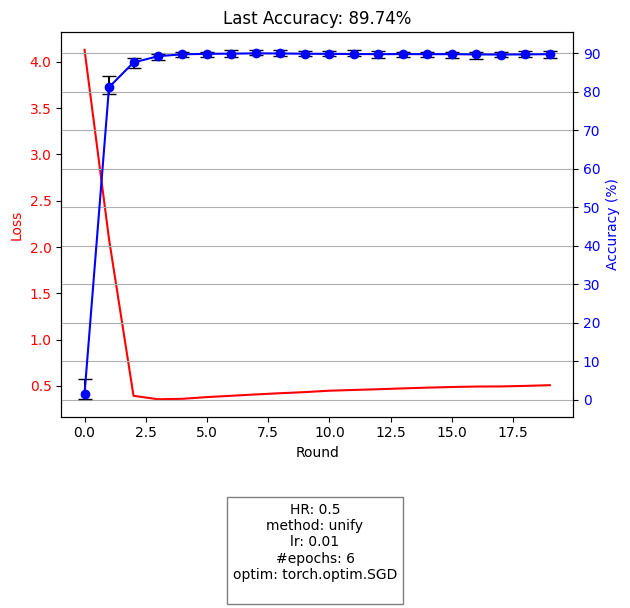
\includegraphics[width=\textwidth]{../plots/femnist-horizontal/sgd/results-h0_5-hm_unify-lr0_01-e6-torch_optim_SGD.png}
    \end{subfigure}
\end{figure}
\begin{figure}[htbp]  % h: here, t: top, b: bottom, p: page
    \centering
    \begin{subfigure}[b]{0.47\textwidth}
        \centering
        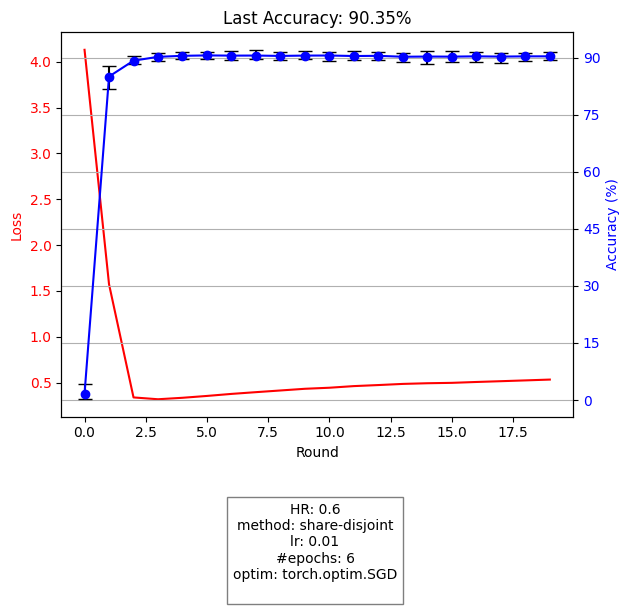
\includegraphics[width=\textwidth]{../plots/femnist-horizontal/sgd/results-h0_6-hm_share-disjoint-lr0_01-e6-torch_optim_SGD.png}
    \end{subfigure}
    \hfill
    \begin{subfigure}[b]{0.47\textwidth}
        \centering
        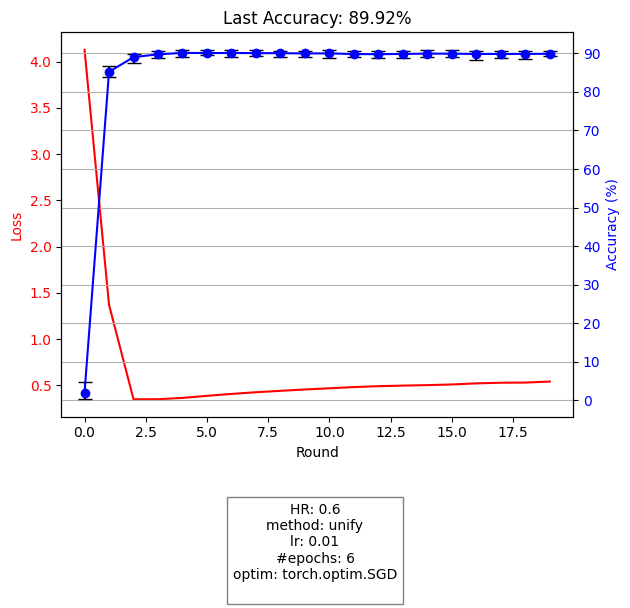
\includegraphics[width=\textwidth]{../plots/femnist-horizontal/sgd/results-h0_6-hm_unify-lr0_01-e6-torch_optim_SGD.png}
    \end{subfigure}
\end{figure}
\begin{figure}[htbp]  % h: here, t: top, b: bottom, p: page
    \centering
    \begin{subfigure}[b]{0.47\textwidth}
        \centering
        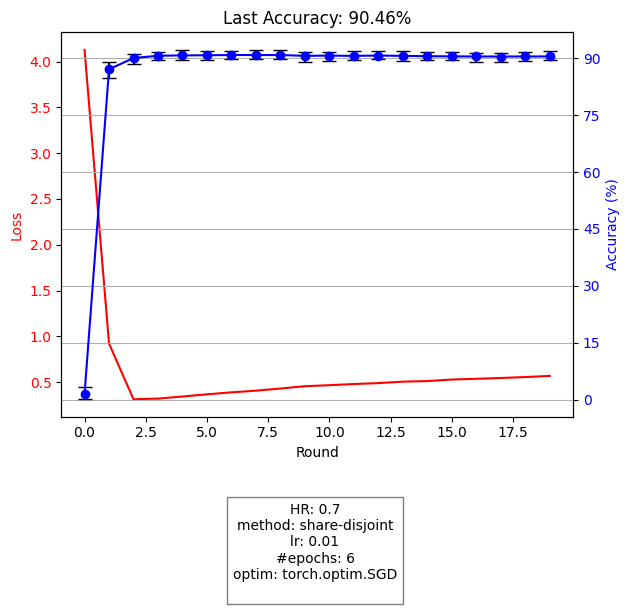
\includegraphics[width=\textwidth]{../plots/femnist-horizontal/sgd/results-h0_7-hm_share-disjoint-lr0_01-e6-torch_optim_SGD.png}
    \end{subfigure}
    \hfill
    \begin{subfigure}[b]{0.47\textwidth}
        \centering
        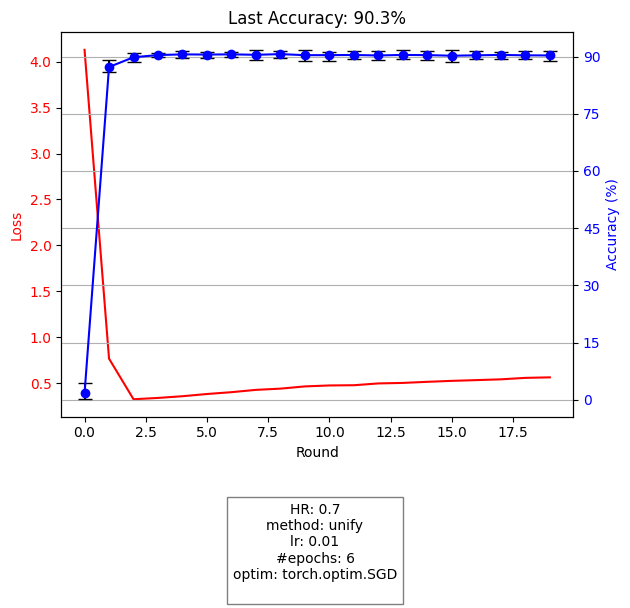
\includegraphics[width=\textwidth]{../plots/femnist-horizontal/sgd/results-h0_7-hm_unify-lr0_01-e6-torch_optim_SGD.png}
    \end{subfigure}
\end{figure}
\begin{figure}[htbp]  % h: here, t: top, b: bottom, p: page
    \centering
    \begin{subfigure}[b]{0.47\textwidth}
        \centering
        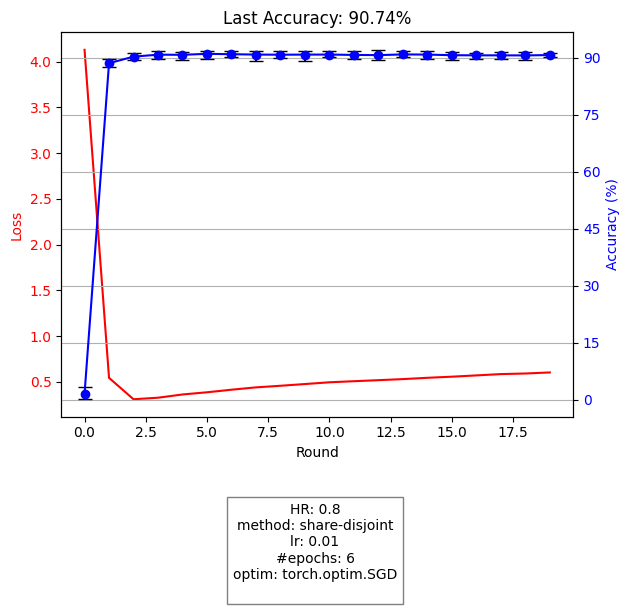
\includegraphics[width=\textwidth]{../plots/femnist-horizontal/sgd/results-h0_8-hm_share-disjoint-lr0_01-e6-torch_optim_SGD.png}
    \end{subfigure}
    \hfill
    \begin{subfigure}[b]{0.47\textwidth}
        \centering
        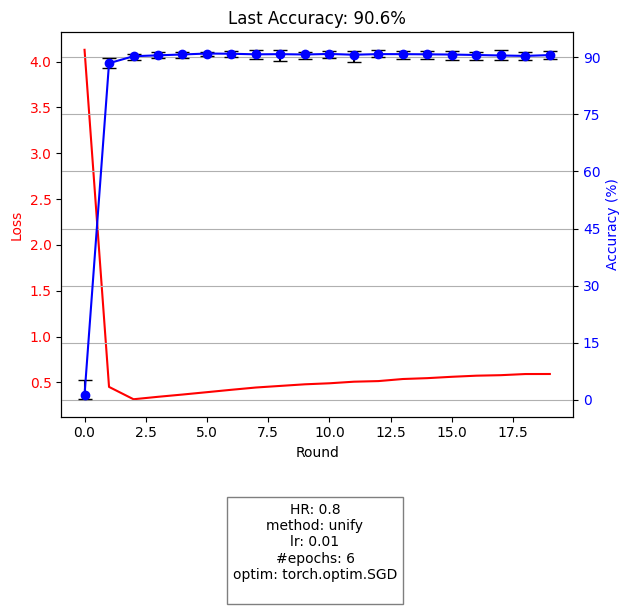
\includegraphics[width=\textwidth]{../plots/femnist-horizontal/sgd/results-h0_8-hm_unify-lr0_01-e6-torch_optim_SGD.png}
    \end{subfigure}
\end{figure}
\begin{figure}[htbp]  % h: here, t: top, b: bottom, p: page
    \centering
    \begin{subfigure}[b]{0.47\textwidth}
        \centering
        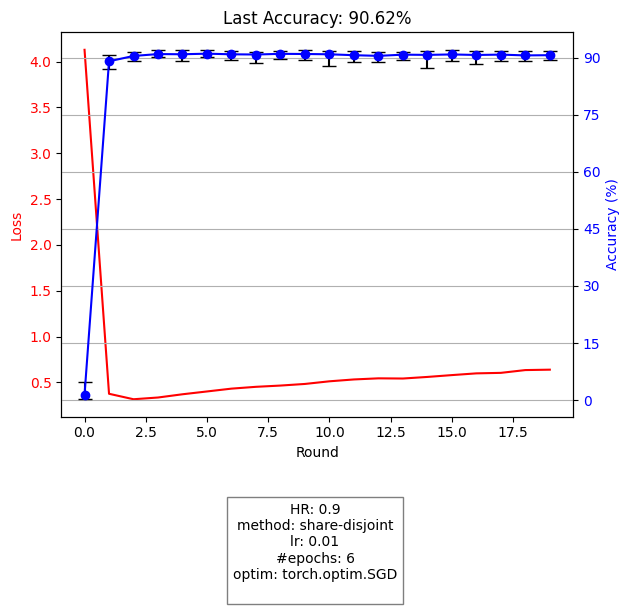
\includegraphics[width=\textwidth]{../plots/femnist-horizontal/sgd/results-h0_9-hm_share-disjoint-lr0_01-e6-torch_optim_SGD.png}
    \end{subfigure}
    \hfill
    \begin{subfigure}[b]{0.47\textwidth}
        \centering
        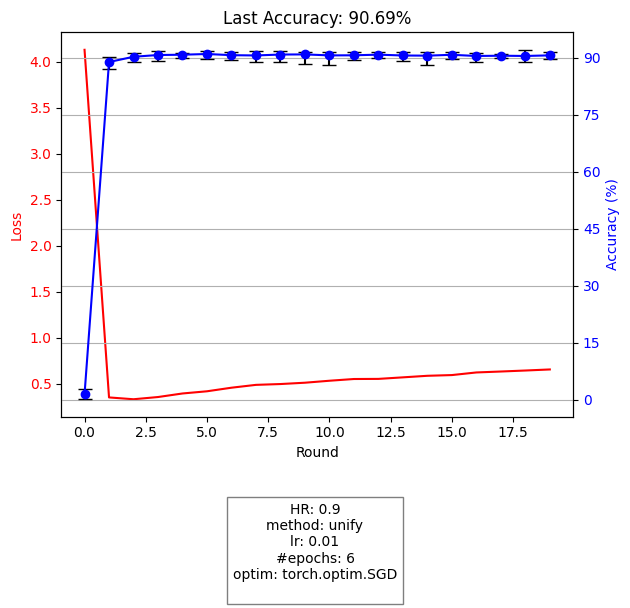
\includegraphics[width=\textwidth]{../plots/femnist-horizontal/sgd/results-h0_9-hm_unify-lr0_01-e6-torch_optim_SGD.png}
    \end{subfigure}
\end{figure}
\begin{figure}[htbp]  % h: here, t: top, b: bottom, p: page
    \centering
    \begin{subfigure}[b]{0.47\textwidth}
        \centering
        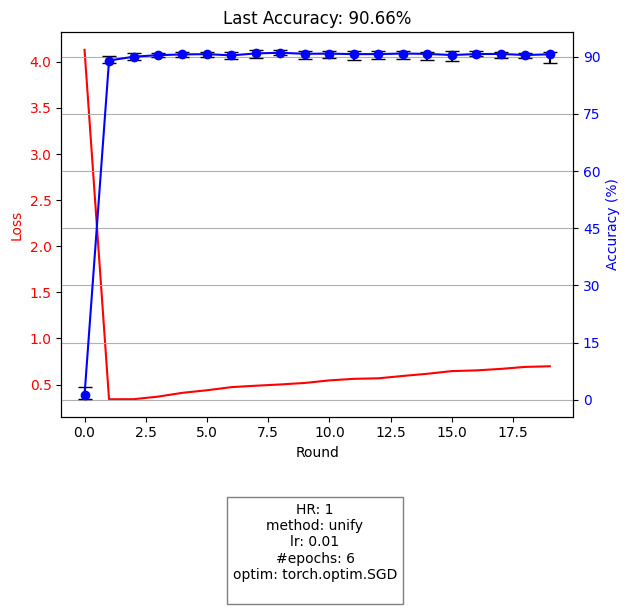
\includegraphics[width=\textwidth]{../plots/femnist-horizontal/sgd/results-h0_10-hm_share-disjoint-lr0_01-e6-torch_optim_SGD.png}
    \end{subfigure}
    \hfill
    \begin{subfigure}[b]{0.47\textwidth}
        \centering
        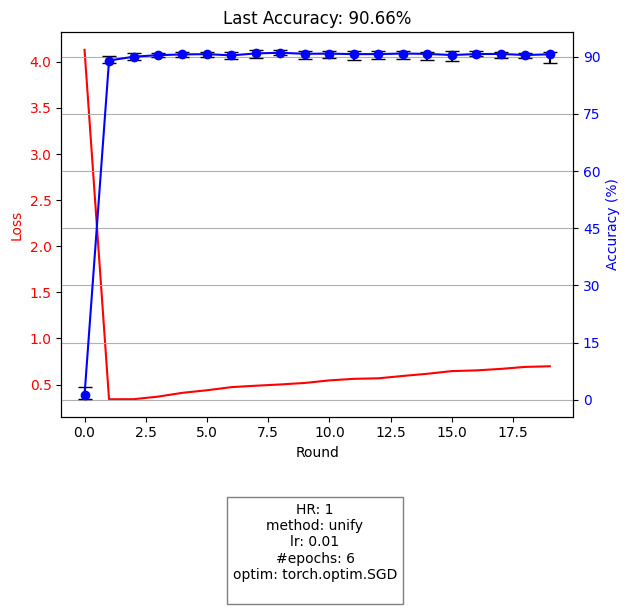
\includegraphics[width=\textwidth]{../plots/femnist-horizontal/sgd/results-h0_10-hm_unify-lr0_01-e6-torch_optim_SGD.png}
    \end{subfigure}
\end{figure}


\clearpage
Ora sono riportati i risultati di AdamW.
\begin{figure}[htbp]  % h: here, t: top, b: bottom, p: page
    \centering
    \begin{subfigure}[b]{0.47\textwidth}
        \centering
        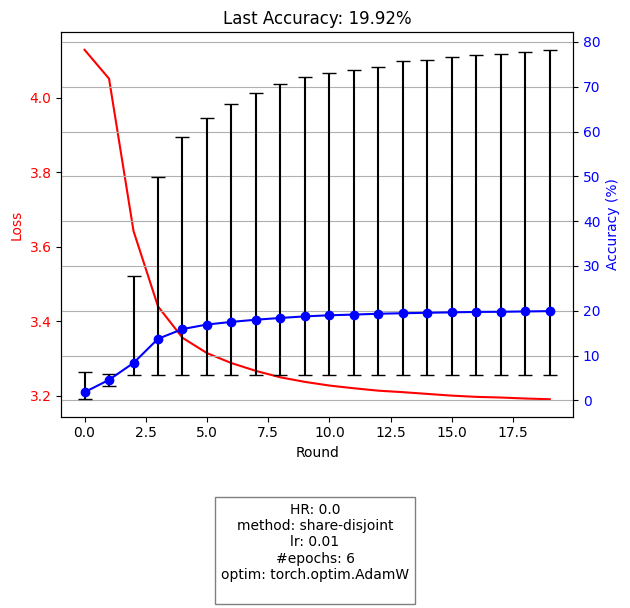
\includegraphics[width=\textwidth]{../plots/femnist-horizontal/adamw/results-h0_0-hm_share-disjoint-lr0_01-e6-torch_optim_AdamW.png}
    \end{subfigure}
    \hfill
    \begin{subfigure}[b]{0.47\textwidth}
        \centering
        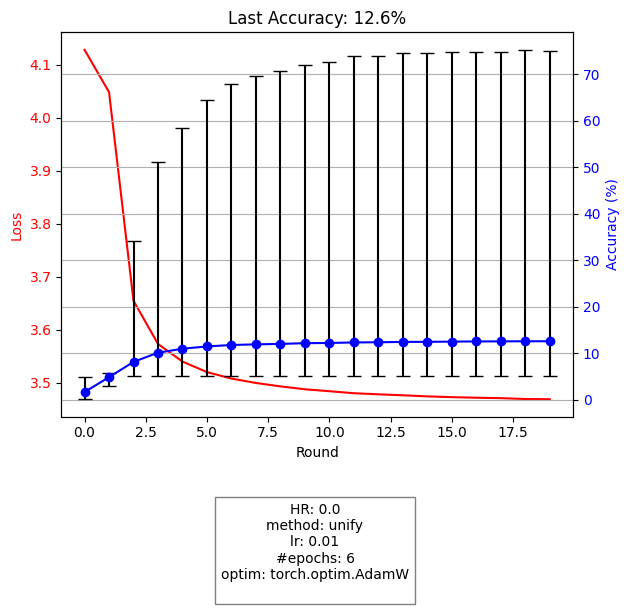
\includegraphics[width=\textwidth]{../plots/femnist-horizontal/adamw/results-h0_0-hm_unify-lr0_01-e6-torch_optim_AdamW.png}
    \end{subfigure}
\end{figure}
\begin{figure}[htbp]  % h: here, t: top, b: bottom, p: page
    \centering
    \begin{subfigure}[b]{0.47\textwidth}
        \centering
        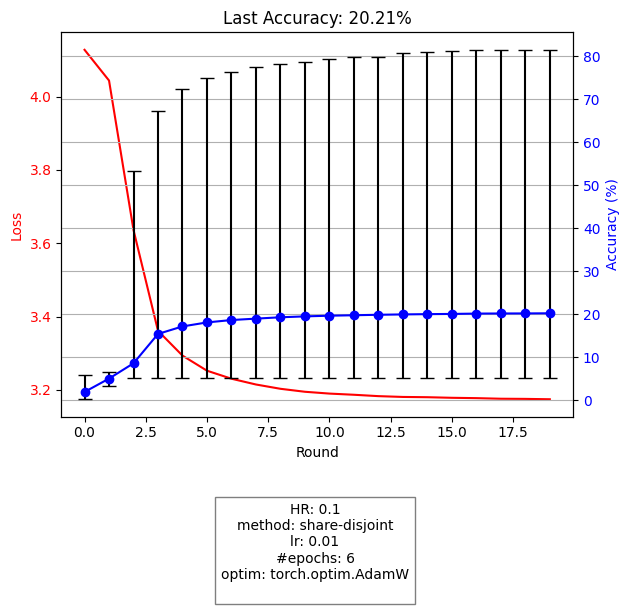
\includegraphics[width=\textwidth]{../plots/femnist-horizontal/adamw/results-h0_1-hm_share-disjoint-lr0_01-e6-torch_optim_AdamW.png}
    \end{subfigure}
    \hfill
    \begin{subfigure}[b]{0.47\textwidth}
        \centering
        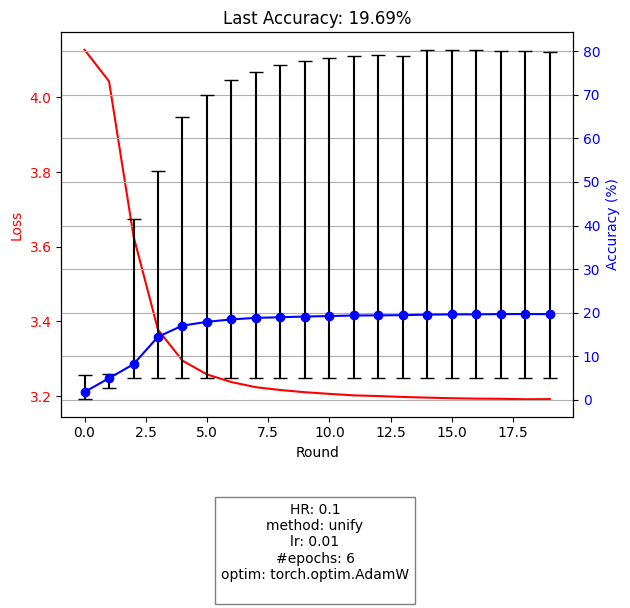
\includegraphics[width=\textwidth]{../plots/femnist-horizontal/adamw/results-h0_1-hm_unify-lr0_01-e6-torch_optim_AdamW.png}
    \end{subfigure}
\end{figure}
\begin{figure}[htbp]  % h: here, t: top, b: bottom, p: page
    \centering
    \begin{subfigure}[b]{0.47\textwidth}
        \centering
        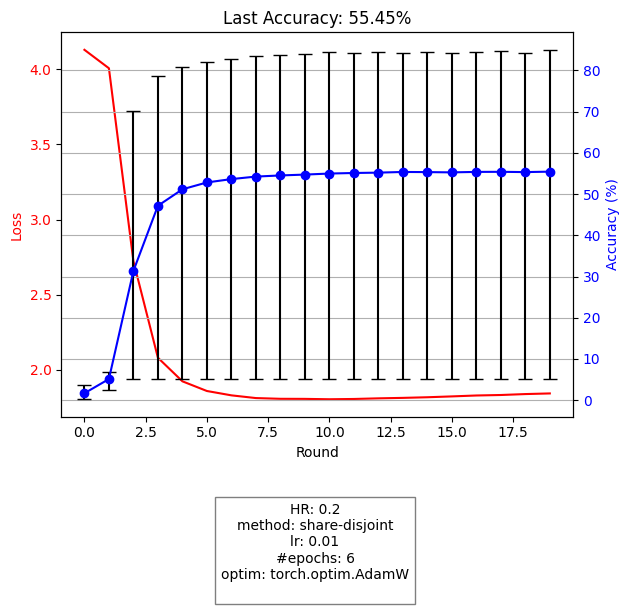
\includegraphics[width=\textwidth]{../plots/femnist-horizontal/adamw/results-h0_2-hm_share-disjoint-lr0_01-e6-torch_optim_AdamW.png}
    \end{subfigure}
    \hfill
    \begin{subfigure}[b]{0.47\textwidth}
        \centering
        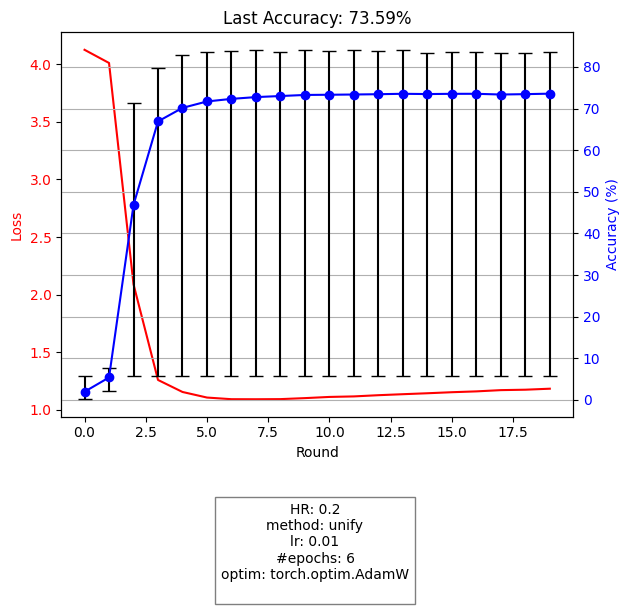
\includegraphics[width=\textwidth]{../plots/femnist-horizontal/adamw/results-h0_2-hm_unify-lr0_01-e6-torch_optim_AdamW.png}
    \end{subfigure}
\end{figure}
\begin{figure}[htbp]  % h: here, t: top, b: bottom, p: page
    \centering
    \begin{subfigure}[b]{0.47\textwidth}
        \centering
        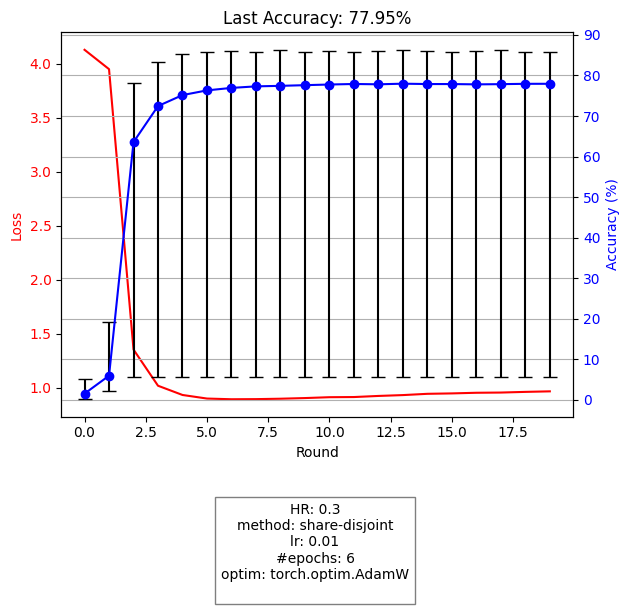
\includegraphics[width=\textwidth]{../plots/femnist-horizontal/adamw/results-h0_3-hm_share-disjoint-lr0_01-e6-torch_optim_AdamW.png}
    \end{subfigure}
    \hfill
    \begin{subfigure}[b]{0.47\textwidth}
        \centering
        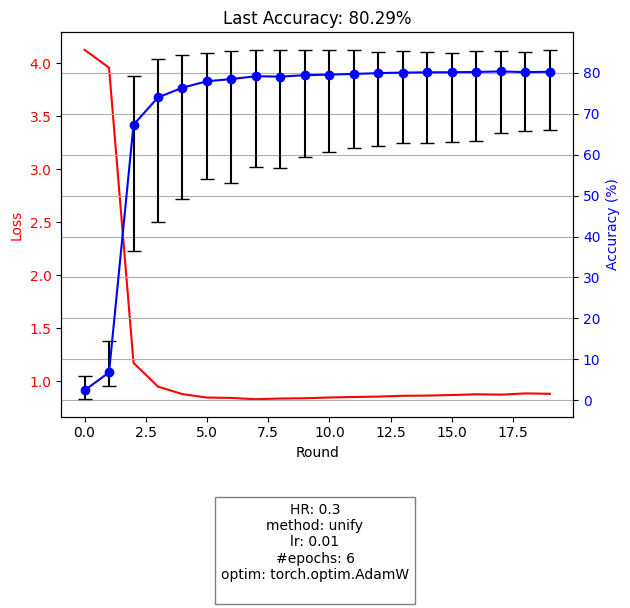
\includegraphics[width=\textwidth]{../plots/femnist-horizontal/adamw/results-h0_3-hm_unify-lr0_01-e6-torch_optim_AdamW.png}
    \end{subfigure}
\end{figure}
\begin{figure}[htbp]  % h: here, t: top, b: bottom, p: page
    \centering
    \begin{subfigure}[b]{0.47\textwidth}
        \centering
        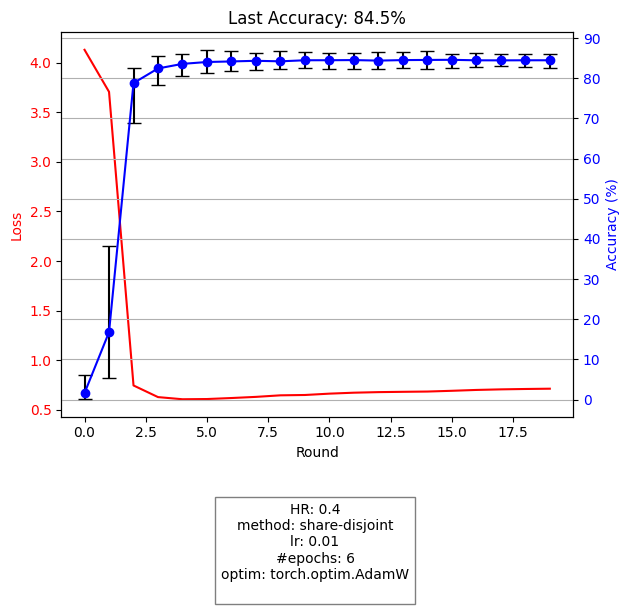
\includegraphics[width=\textwidth]{../plots/femnist-horizontal/adamw/results-h0_4-hm_share-disjoint-lr0_01-e6-torch_optim_AdamW.png}
    \end{subfigure}
    \hfill
    \begin{subfigure}[b]{0.47\textwidth}
        \centering
        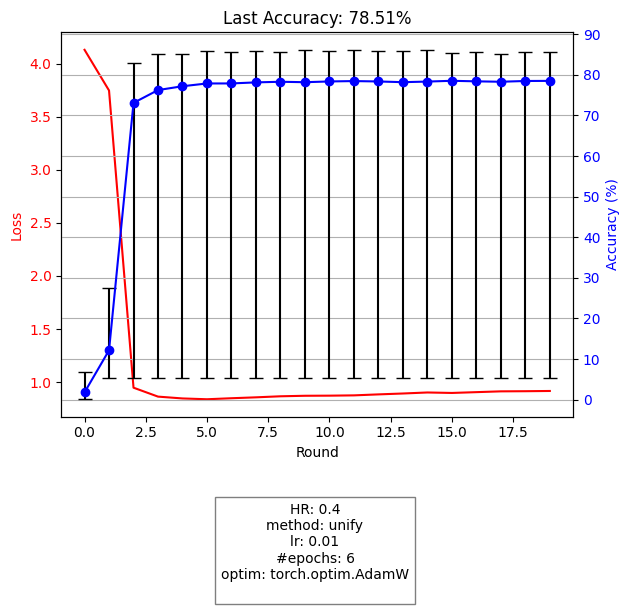
\includegraphics[width=\textwidth]{../plots/femnist-horizontal/adamw/results-h0_4-hm_unify-lr0_01-e6-torch_optim_AdamW.png}
    \end{subfigure}
\end{figure}
\begin{figure}[htbp]  % h: here, t: top, b: bottom, p: page
    \centering
    \begin{subfigure}[b]{0.47\textwidth}
        \centering
        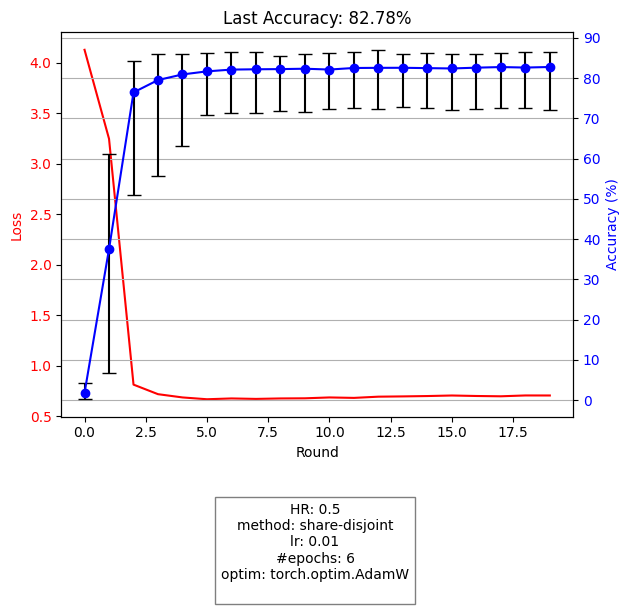
\includegraphics[width=\textwidth]{../plots/femnist-horizontal/adamw/results-h0_5-hm_share-disjoint-lr0_01-e6-torch_optim_AdamW.png}
    \end{subfigure}
    \hfill
    \begin{subfigure}[b]{0.47\textwidth}
        \centering
        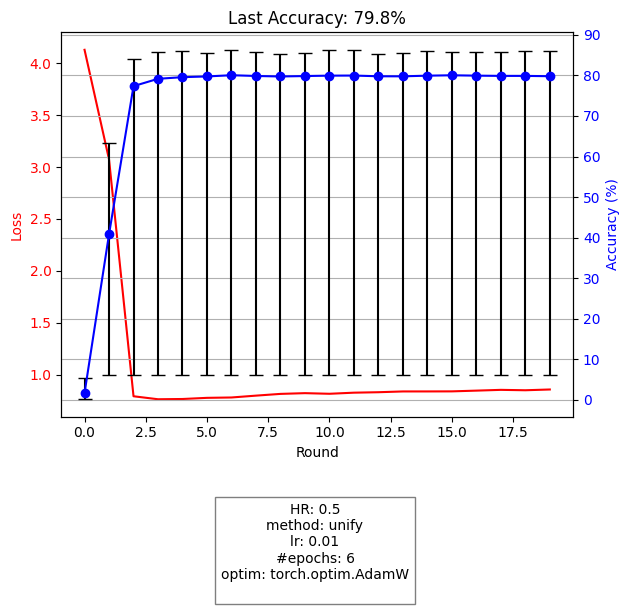
\includegraphics[width=\textwidth]{../plots/femnist-horizontal/adamw/results-h0_5-hm_unify-lr0_01-e6-torch_optim_AdamW.png}
    \end{subfigure}
\end{figure}
\begin{figure}[htbp]  % h: here, t: top, b: bottom, p: page
    \centering
    \begin{subfigure}[b]{0.47\textwidth}
        \centering
        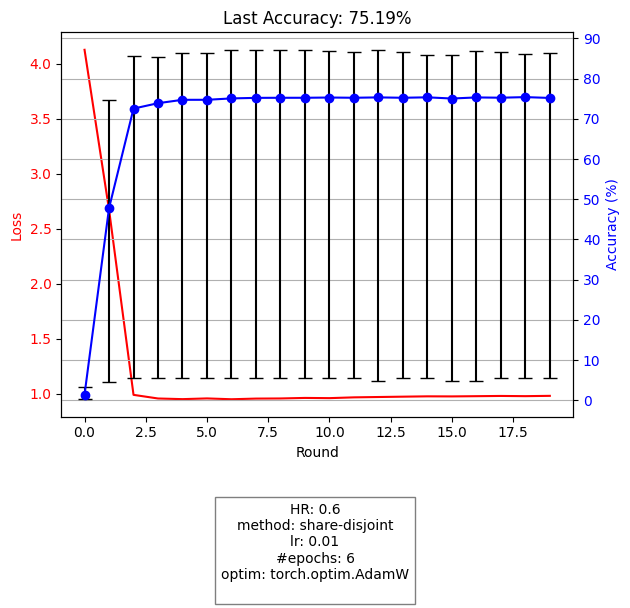
\includegraphics[width=\textwidth]{../plots/femnist-horizontal/adamw/results-h0_6-hm_share-disjoint-lr0_01-e6-torch_optim_AdamW.png}
    \end{subfigure}
    \hfill
    \begin{subfigure}[b]{0.47\textwidth}
        \centering
        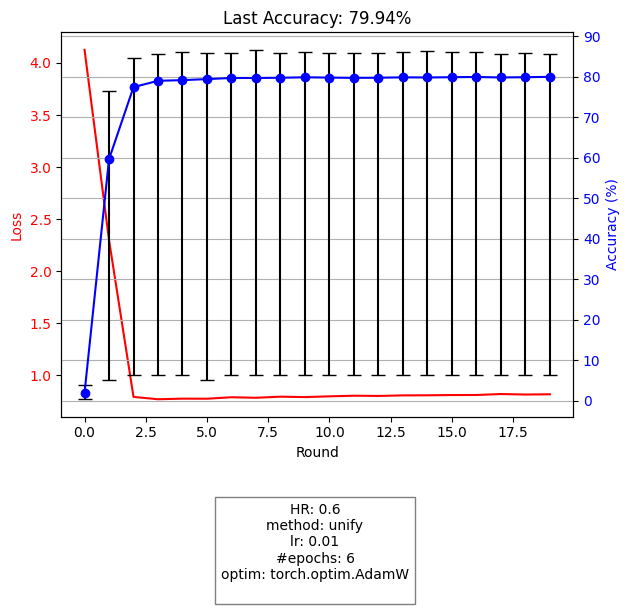
\includegraphics[width=\textwidth]{../plots/femnist-horizontal/adamw/results-h0_6-hm_unify-lr0_01-e6-torch_optim_AdamW.png}
    \end{subfigure}
\end{figure}
\begin{figure}[htbp]  % h: here, t: top, b: bottom, p: page
    \centering
    \begin{subfigure}[b]{0.47\textwidth}
        \centering
        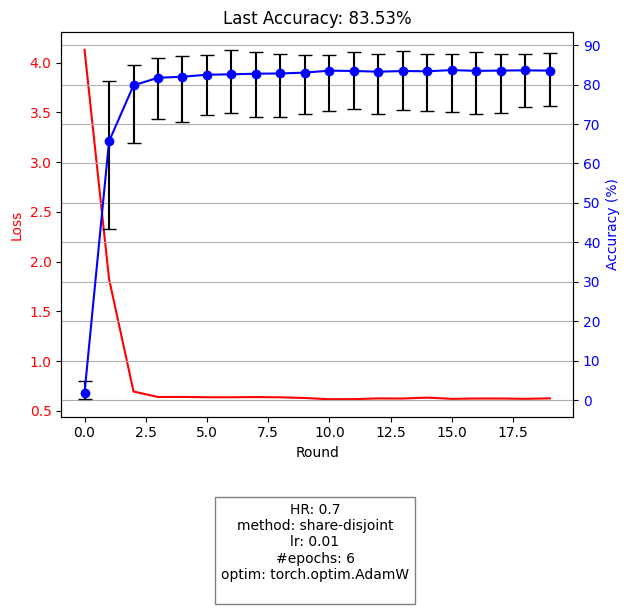
\includegraphics[width=\textwidth]{../plots/femnist-horizontal/adamw/results-h0_7-hm_share-disjoint-lr0_01-e6-torch_optim_AdamW.png}
    \end{subfigure}
    \hfill
    \begin{subfigure}[b]{0.47\textwidth}
        \centering
        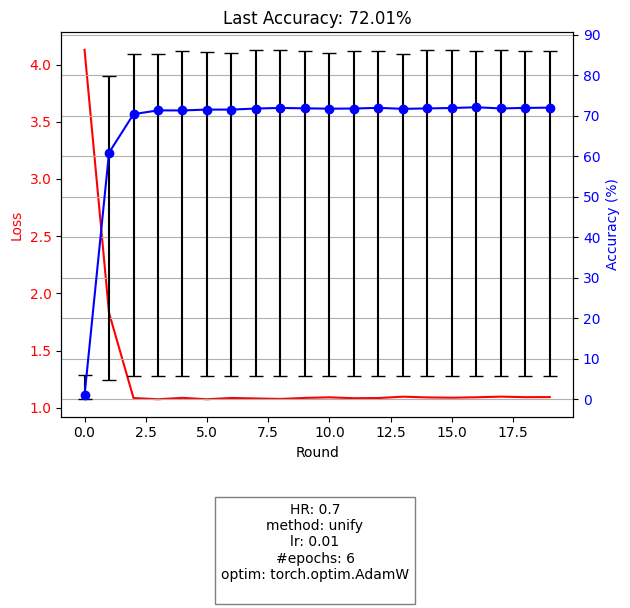
\includegraphics[width=\textwidth]{../plots/femnist-horizontal/adamw/results-h0_7-hm_unify-lr0_01-e6-torch_optim_AdamW.png}
    \end{subfigure}
\end{figure}
\begin{figure}[htbp]  % h: here, t: top, b: bottom, p: page
    \centering
    \begin{subfigure}[b]{0.47\textwidth}
        \centering
        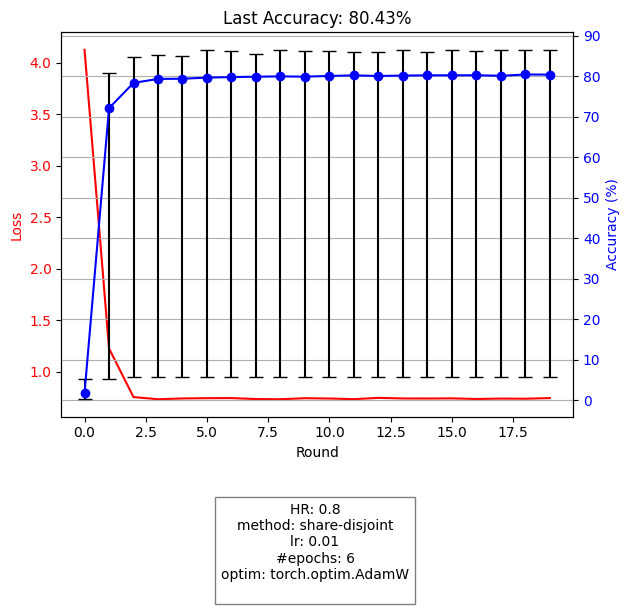
\includegraphics[width=\textwidth]{../plots/femnist-horizontal/adamw/results-h0_8-hm_share-disjoint-lr0_01-e6-torch_optim_AdamW.png}
    \end{subfigure}
    \hfill
    \begin{subfigure}[b]{0.47\textwidth}
        \centering
        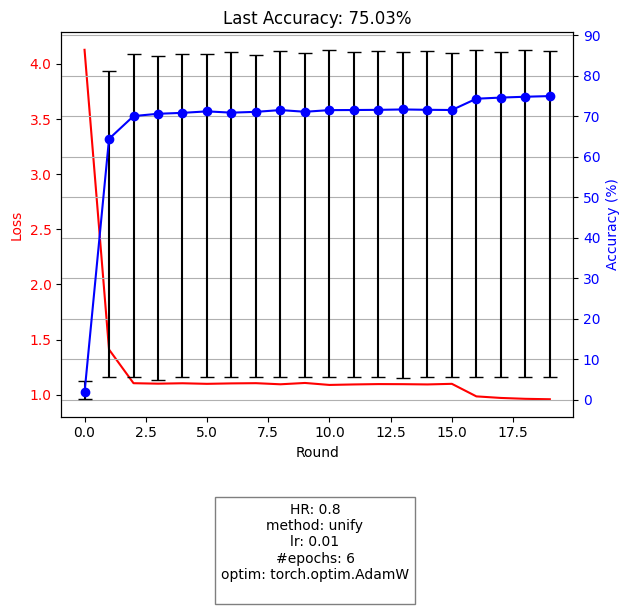
\includegraphics[width=\textwidth]{../plots/femnist-horizontal/adamw/results-h0_8-hm_unify-lr0_01-e6-torch_optim_AdamW.png}
    \end{subfigure}
\end{figure}
\begin{figure}[htbp]  % h: here, t: top, b: bottom, p: page
    \centering
    \begin{subfigure}[b]{0.47\textwidth}
        \centering
        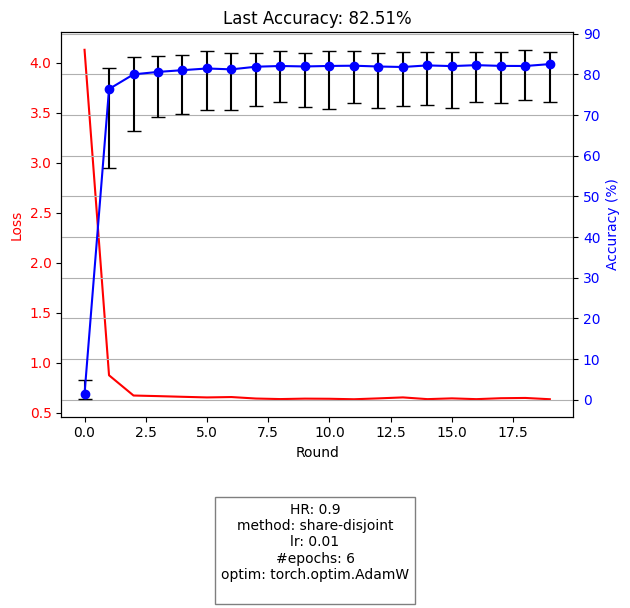
\includegraphics[width=\textwidth]{../plots/femnist-horizontal/adamw/results-h0_9-hm_share-disjoint-lr0_01-e6-torch_optim_AdamW.png}
    \end{subfigure}
    \hfill
    \begin{subfigure}[b]{0.47\textwidth}
        \centering
        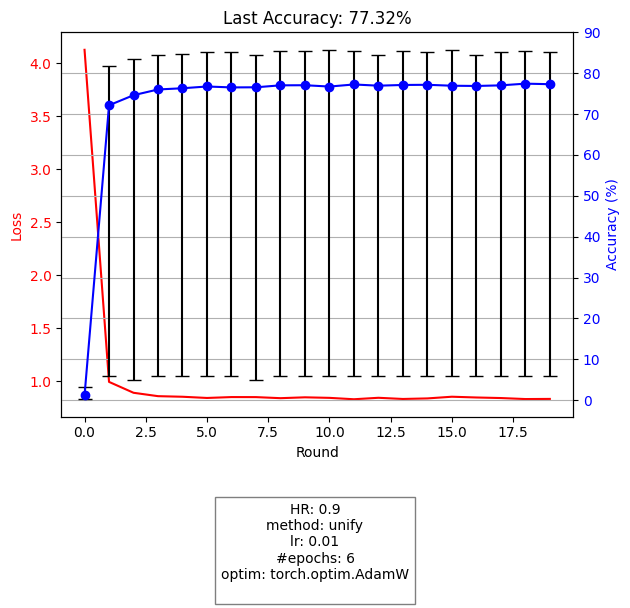
\includegraphics[width=\textwidth]{../plots/femnist-horizontal/adamw/results-h0_9-hm_unify-lr0_01-e6-torch_optim_AdamW.png}
    \end{subfigure}
\end{figure}
\begin{figure}[htbp]  % h: here, t: top, b: bottom, p: page
    \centering
    \begin{subfigure}[b]{0.47\textwidth}
        \centering
        \includegraphics[width=\textwidth]{../plots/femnist-horizontal/adamw/results-h0_10-hm_share-disjoint-lr0_01-e6-torch_optim_AdamW.png}
    \end{subfigure}
    \hfill
    \begin{subfigure}[b]{0.47\textwidth}
        \centering
        \includegraphics[width=\textwidth]{../plots/femnist-horizontal/adamw/results-h0_10-hm_unify-lr0_01-e6-torch_optim_AdamW.png}
    \end{subfigure}
\end{figure}

\chapter{Appendix B - Grafici UCI HAR}
Anche per questo dataset, qui di seguito si trovano i grafici dei
risultati di tutti gli esperimenti condotti. La colonna di sinistra 
riporta i risultati ottenuti con il metodo \texttt{share-disjoint}, 
quella di destra \texttt{unify}. Sono prima riportati i risultati 
di SGD.

\begin{figure}[htbp]  % h: here, t: top, b: bottom, p: page
    \centering
    \begin{subfigure}[b]{0.47\textwidth}
        \centering
        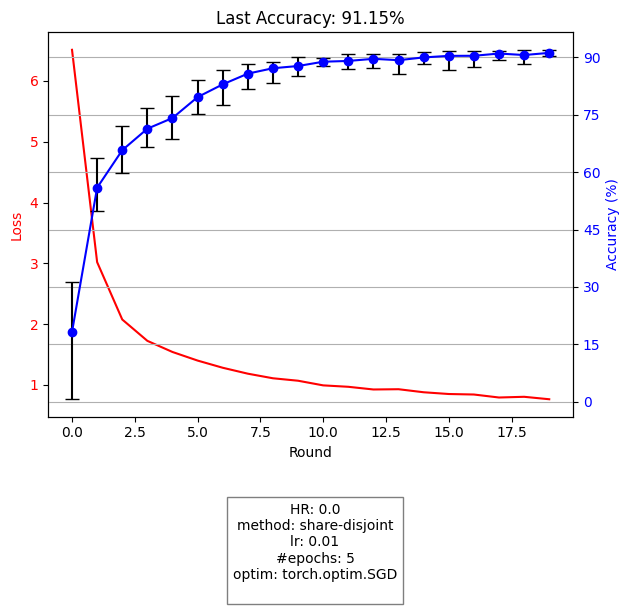
\includegraphics[width=\textwidth]{../plots/har-horizontal/sgd/results-h0_0-hm_share-disjoint-lr0_01-e5-torch_optim_SGD.png}
    \end{subfigure}
    \hfill
    \begin{subfigure}[b]{0.47\textwidth}
        \centering
        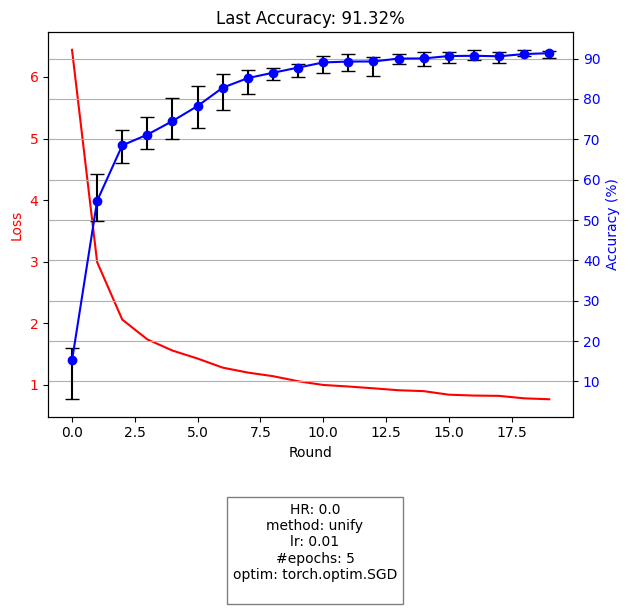
\includegraphics[width=\textwidth]{../plots/har-horizontal/sgd/results-h0_0-hm_unify-lr0_01-e5-torch_optim_SGD.png}
    \end{subfigure}
\end{figure}
\begin{figure}[htbp]  % h: here, t: top, b: bottom, p: page
    \centering
    \begin{subfigure}[b]{0.47\textwidth}
        \centering
        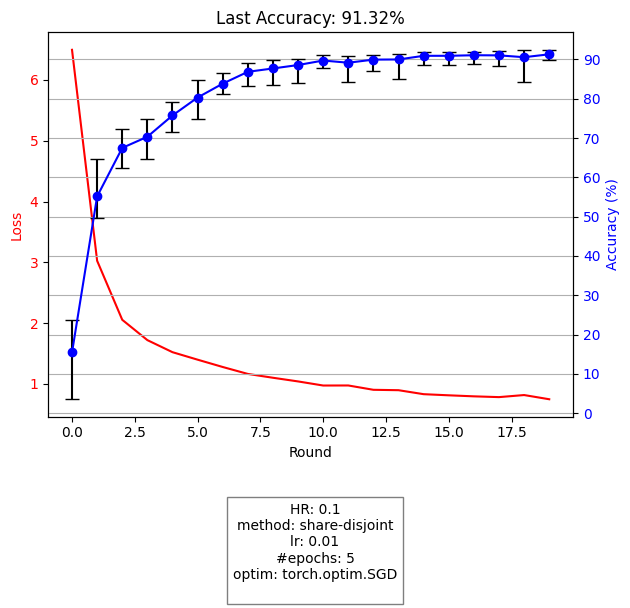
\includegraphics[width=\textwidth]{../plots/har-horizontal/sgd/results-h0_1-hm_share-disjoint-lr0_01-e5-torch_optim_SGD.png}
    \end{subfigure}
    \hfill
    \begin{subfigure}[b]{0.47\textwidth}
        \centering
        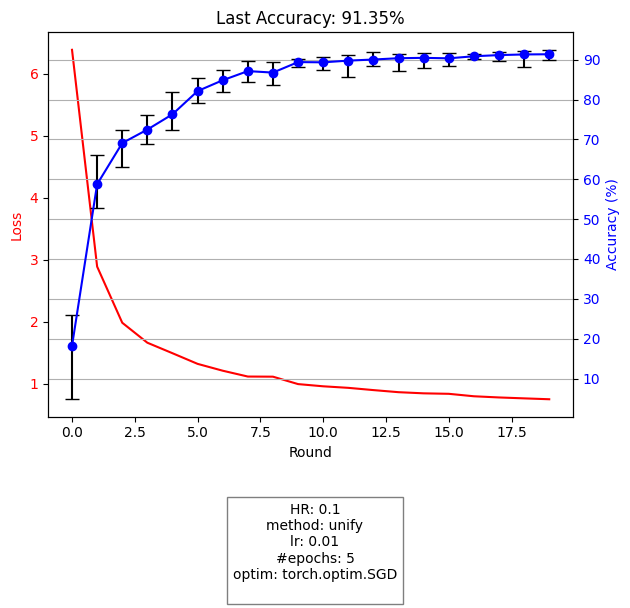
\includegraphics[width=\textwidth]{../plots/har-horizontal/sgd/results-h0_1-hm_unify-lr0_01-e5-torch_optim_SGD.png}
    \end{subfigure}
\end{figure}
\begin{figure}[htbp]  % h: here, t: top, b: bottom, p: page
    \centering
    \begin{subfigure}[b]{0.47\textwidth}
        \centering
        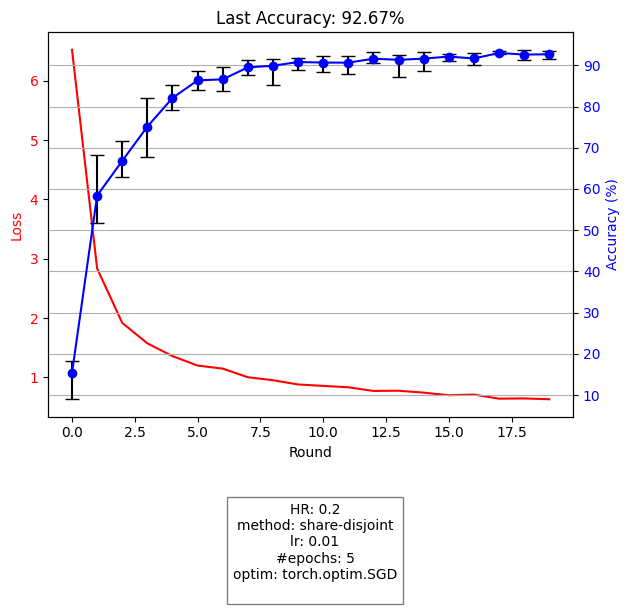
\includegraphics[width=\textwidth]{../plots/har-horizontal/sgd/results-h0_2-hm_share-disjoint-lr0_01-e5-torch_optim_SGD.png}
    \end{subfigure}
    \hfill
    \begin{subfigure}[b]{0.47\textwidth}
        \centering
        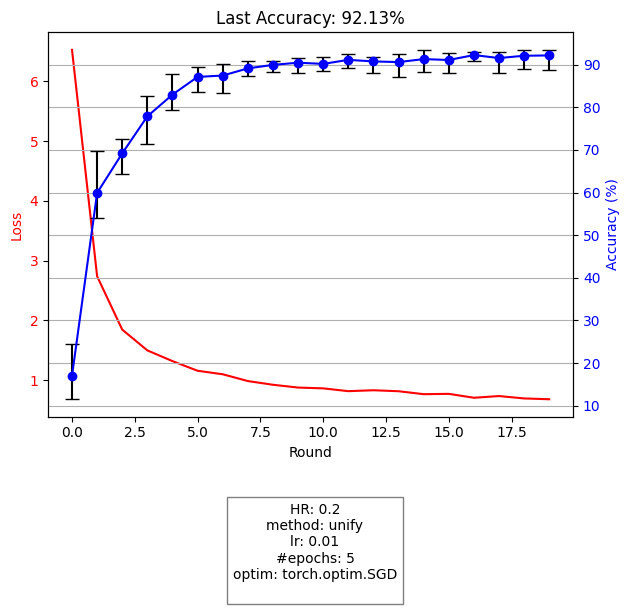
\includegraphics[width=\textwidth]{../plots/har-horizontal/sgd/results-h0_2-hm_unify-lr0_01-e5-torch_optim_SGD.png}
    \end{subfigure}
\end{figure}
\begin{figure}[htbp]  % h: here, t: top, b: bottom, p: page
    \centering
    \begin{subfigure}[b]{0.47\textwidth}
        \centering
        \includegraphics[width=\textwidth]{../plots/har-horizontal/sgd/results-h0_3-hm_share-disjoint-lr0_01-e5-torch_optim_SGD.png}
    \end{subfigure}
    \hfill
    \begin{subfigure}[b]{0.47\textwidth}
        \centering
        \includegraphics[width=\textwidth]{../plots/har-horizontal/sgd/results-h0_3-hm_unify-lr0_01-e5-torch_optim_SGD.png}
    \end{subfigure}
\end{figure}
\begin{figure}[htbp]  % h: here, t: top, b: bottom, p: page
    \centering
    \begin{subfigure}[b]{0.47\textwidth}
        \centering
        \includegraphics[width=\textwidth]{../plots/har-horizontal/sgd/results-h0_4-hm_share-disjoint-lr0_01-e5-torch_optim_SGD.png}
    \end{subfigure}
    \hfill
    \begin{subfigure}[b]{0.47\textwidth}
        \centering
        \includegraphics[width=\textwidth]{../plots/har-horizontal/sgd/results-h0_4-hm_unify-lr0_01-e5-torch_optim_SGD.png}
    \end{subfigure}
\end{figure}
\begin{figure}[htbp]  % h: here, t: top, b: bottom, p: page
    \centering
    \begin{subfigure}[b]{0.47\textwidth}
        \centering
        \includegraphics[width=\textwidth]{../plots/har-horizontal/sgd/results-h0_5-hm_share-disjoint-lr0_01-e5-torch_optim_SGD.png}
    \end{subfigure}
    \hfill
    \begin{subfigure}[b]{0.47\textwidth}
        \centering
        \includegraphics[width=\textwidth]{../plots/har-horizontal/sgd/results-h0_5-hm_unify-lr0_01-e5-torch_optim_SGD.png}
    \end{subfigure}
\end{figure}
\begin{figure}[htbp]  % h: here, t: top, b: bottom, p: page
    \centering
    \begin{subfigure}[b]{0.47\textwidth}
        \centering
        \includegraphics[width=\textwidth]{../plots/har-horizontal/sgd/results-h0_6-hm_share-disjoint-lr0_01-e5-torch_optim_SGD.png}
    \end{subfigure}
    \hfill
    \begin{subfigure}[b]{0.47\textwidth}
        \centering
        \includegraphics[width=\textwidth]{../plots/har-horizontal/sgd/results-h0_6-hm_unify-lr0_01-e5-torch_optim_SGD.png}
    \end{subfigure}
\end{figure}
\begin{figure}[htbp]  % h: here, t: top, b: bottom, p: page
    \centering
    \begin{subfigure}[b]{0.47\textwidth}
        \centering
        \includegraphics[width=\textwidth]{../plots/har-horizontal/sgd/results-h0_7-hm_share-disjoint-lr0_01-e5-torch_optim_SGD.png}
    \end{subfigure}
    \hfill
    \begin{subfigure}[b]{0.47\textwidth}
        \centering
        \includegraphics[width=\textwidth]{../plots/har-horizontal/sgd/results-h0_7-hm_unify-lr0_01-e5-torch_optim_SGD.png}
    \end{subfigure}
\end{figure}
\begin{figure}[htbp]  % h: here, t: top, b: bottom, p: page
    \centering
    \begin{subfigure}[b]{0.47\textwidth}
        \centering
        \includegraphics[width=\textwidth]{../plots/har-horizontal/sgd/results-h0_8-hm_share-disjoint-lr0_01-e5-torch_optim_SGD.png}
    \end{subfigure}
    \hfill
    \begin{subfigure}[b]{0.47\textwidth}
        \centering
        \includegraphics[width=\textwidth]{../plots/har-horizontal/sgd/results-h0_8-hm_unify-lr0_01-e5-torch_optim_SGD.png}
    \end{subfigure}
\end{figure}
\begin{figure}[htbp]  % h: here, t: top, b: bottom, p: page
    \centering
    \begin{subfigure}[b]{0.47\textwidth}
        \centering
        \includegraphics[width=\textwidth]{../plots/har-horizontal/sgd/results-h0_9-hm_share-disjoint-lr0_01-e5-torch_optim_SGD.png}
    \end{subfigure}
    \hfill
    \begin{subfigure}[b]{0.47\textwidth}
        \centering
        \includegraphics[width=\textwidth]{../plots/har-horizontal/sgd/results-h0_9-hm_unify-lr0_01-e5-torch_optim_SGD.png}
    \end{subfigure}
\end{figure}
\begin{figure}[htbp]  % h: here, t: top, b: bottom, p: page
    \centering
    \begin{subfigure}[b]{0.47\textwidth}
        \centering
        \includegraphics[width=\textwidth]{../plots/har-horizontal/sgd/results-h0_10-hm_share-disjoint-lr0_01-e6-torch_optim_SGD.png}
    \end{subfigure}
    \hfill
    \begin{subfigure}[b]{0.47\textwidth}
        \centering
        \includegraphics[width=\textwidth]{../plots/har-horizontal/sgd/results-h0_10-hm_unify-lr0_01-e6-torch_optim_SGD.png}
    \end{subfigure}
\end{figure}


\clearpage
I seguenti sono i risultati di AdamW.
\begin{figure}[htbp]  % h: here, t: top, b: bottom, p: page
    \centering
    \begin{subfigure}[b]{0.47\textwidth}
        \centering
        \includegraphics[width=\textwidth]{../plots/har-horizontal/adam/results-h0_0-hm_share-disjoint-lr0_01-e5-torch_optim_AdamW.png}
    \end{subfigure}
    \hfill
    \begin{subfigure}[b]{0.47\textwidth}
        \centering
        \includegraphics[width=\textwidth]{../plots/har-horizontal/adam/results-h0_0-hm_unify-lr0_01-e5-torch_optim_AdamW.png}
    \end{subfigure}
\end{figure}
\begin{figure}[htbp]  % h: here, t: top, b: bottom, p: page
    \centering
    \begin{subfigure}[b]{0.47\textwidth}
        \centering
        \includegraphics[width=\textwidth]{../plots/har-horizontal/adam/results-h0_1-hm_share-disjoint-lr0_01-e5-torch_optim_AdamW.png}
    \end{subfigure}
    \hfill
    \begin{subfigure}[b]{0.47\textwidth}
        \centering
        \includegraphics[width=\textwidth]{../plots/har-horizontal/adam/results-h0_1-hm_unify-lr0_01-e5-torch_optim_AdamW.png}
    \end{subfigure}
\end{figure}
\begin{figure}[htbp]  % h: here, t: top, b: bottom, p: page
    \centering
    \begin{subfigure}[b]{0.47\textwidth}
        \centering
        \includegraphics[width=\textwidth]{../plots/har-horizontal/adam/results-h0_2-hm_share-disjoint-lr0_01-e5-torch_optim_AdamW.png}
    \end{subfigure}
    \hfill
    \begin{subfigure}[b]{0.47\textwidth}
        \centering
        \includegraphics[width=\textwidth]{../plots/har-horizontal/adam/results-h0_2-hm_unify-lr0_01-e5-torch_optim_AdamW.png}
    \end{subfigure}
\end{figure}
\begin{figure}[htbp]  % h: here, t: top, b: bottom, p: page
    \centering
    \begin{subfigure}[b]{0.47\textwidth}
        \centering
        \includegraphics[width=\textwidth]{../plots/har-horizontal/adam/results-h0_3-hm_share-disjoint-lr0_01-e5-torch_optim_AdamW.png}
    \end{subfigure}
    \hfill
    \begin{subfigure}[b]{0.47\textwidth}
        \centering
        \includegraphics[width=\textwidth]{../plots/har-horizontal/adam/results-h0_3-hm_unify-lr0_01-e5-torch_optim_AdamW.png}
    \end{subfigure}
\end{figure}
\begin{figure}[htbp]  % h: here, t: top, b: bottom, p: page
    \centering
    \begin{subfigure}[b]{0.47\textwidth}
        \centering
        \includegraphics[width=\textwidth]{../plots/har-horizontal/adam/results-h0_4-hm_share-disjoint-lr0_01-e5-torch_optim_AdamW.png}
    \end{subfigure}
    \hfill
    \begin{subfigure}[b]{0.47\textwidth}
        \centering
        \includegraphics[width=\textwidth]{../plots/har-horizontal/adam/results-h0_4-hm_unify-lr0_01-e5-torch_optim_AdamW.png}
    \end{subfigure}
\end{figure}
\begin{figure}[htbp]  % h: here, t: top, b: bottom, p: page
    \centering
    \begin{subfigure}[b]{0.47\textwidth}
        \centering
        \includegraphics[width=\textwidth]{../plots/har-horizontal/adam/results-h0_5-hm_share-disjoint-lr0_01-e5-torch_optim_AdamW.png}
    \end{subfigure}
    \hfill
    \begin{subfigure}[b]{0.47\textwidth}
        \centering
        \includegraphics[width=\textwidth]{../plots/har-horizontal/adam/results-h0_5-hm_unify-lr0_01-e5-torch_optim_AdamW.png}
    \end{subfigure}
\end{figure}
\begin{figure}[htbp]  % h: here, t: top, b: bottom, p: page
    \centering
    \begin{subfigure}[b]{0.47\textwidth}
        \centering
        \includegraphics[width=\textwidth]{../plots/har-horizontal/adam/results-h0_6-hm_share-disjoint-lr0_01-e5-torch_optim_AdamW.png}
    \end{subfigure}
    \hfill
    \begin{subfigure}[b]{0.47\textwidth}
        \centering
        \includegraphics[width=\textwidth]{../plots/har-horizontal/adam/results-h0_6-hm_unify-lr0_01-e5-torch_optim_AdamW.png}
    \end{subfigure}
\end{figure}
\begin{figure}[htbp]  % h: here, t: top, b: bottom, p: page
    \centering
    \begin{subfigure}[b]{0.47\textwidth}
        \centering
        \includegraphics[width=\textwidth]{../plots/har-horizontal/adam/results-h0_7-hm_share-disjoint-lr0_01-e5-torch_optim_AdamW.png}
    \end{subfigure}
    \hfill
    \begin{subfigure}[b]{0.47\textwidth}
        \centering
        \includegraphics[width=\textwidth]{../plots/har-horizontal/adam/results-h0_7-hm_unify-lr0_01-e5-torch_optim_AdamW.png}
    \end{subfigure}
\end{figure}
\begin{figure}[htbp]  % h: here, t: top, b: bottom, p: page
    \centering
    \begin{subfigure}[b]{0.47\textwidth}
        \centering
        \includegraphics[width=\textwidth]{../plots/har-horizontal/adam/results-h0_8-hm_share-disjoint-lr0_01-e5-torch_optim_AdamW.png}
    \end{subfigure}
    \hfill
    \begin{subfigure}[b]{0.47\textwidth}
        \centering
        \includegraphics[width=\textwidth]{../plots/har-horizontal/adam/results-h0_8-hm_unify-lr0_01-e5-torch_optim_AdamW.png}
    \end{subfigure}
\end{figure}
\begin{figure}[htbp]  % h: here, t: top, b: bottom, p: page
    \centering
    \begin{subfigure}[b]{0.47\textwidth}
        \centering
        \includegraphics[width=\textwidth]{../plots/har-horizontal/adam/results-h0_9-hm_share-disjoint-lr0_01-e5-torch_optim_AdamW.png}
    \end{subfigure}
    \hfill
    \begin{subfigure}[b]{0.47\textwidth}
        \centering
        \includegraphics[width=\textwidth]{../plots/har-horizontal/adam/results-h0_9-hm_unify-lr0_01-e5-torch_optim_AdamW.png}
    \end{subfigure}
\end{figure}
\begin{figure}[htbp]  % h: here, t: top, b: bottom, p: page
    \centering
    \begin{subfigure}[b]{0.47\textwidth}
        \centering
        \includegraphics[width=\textwidth]{../plots/har-horizontal/adam/results-h0_10-hm_share-disjoint-lr0_01-e6-torch_optim_AdamW.png}
    \end{subfigure}
    \hfill
    \begin{subfigure}[b]{0.47\textwidth}
        \centering
        \includegraphics[width=\textwidth]{../plots/har-horizontal/adam/results-h0_10-hm_unify-lr0_01-e6-torch_optim_AdamW.png}
    \end{subfigure}
\end{figure}

